\documentclass[a4paper,12pt]{article} % This defines the style of your paper

\usepackage[top = 2.5cm, bottom = 2.5cm, left = 2.5cm, right = 2.5cm]{geometry} 

% Unfortunately, LaTeX has a hard time interpreting German Umlaute. The following two lines and packages should help. If it doesn't work for you please let me know.
\usepackage[T1]{fontenc}
\usepackage[utf8]{inputenc}
\usepackage{pifont}
% \usepackage{ctex}
\usepackage{amsthm, amsmath, amssymb, mathrsfs,mathtools}
% ---------------------------------------------------------------------
% Program: listings-stata.tex
% Author:  github.com/mcaceresb
% Purpose: Stata language definition for LaTeX listings package
% Usage:   Add \input{listings-stata.tex} to your preamble

% Syntax from
% - https://github.com/isagalaev/highlight.js/blob/master/src/languages/stata.js
% - https://github.com/jpitblado/vim-stata/blob/master/syntax/stata.vim
% - http://fmwww.bc.edu/RePEc/bocode/s/synlightlist.ado

\RequirePackage{listings}
\RequirePackage{color}
\RequirePackage[svgnames]{xcolor}
\definecolor{spRed}{HTML}{BE646C}

% ---------------------------------------------------------------------
% Stata language definition

\lstdefinelanguage{stata}{
  sensitive=true,
  %
  % Macros, global and local
  alsoletter={\{\}0123456789},
  keywordsprefix=\$,
  morecomment=[n][keywordstyle9]{`}{'},
  morekeywords={},
  %
  % Comments
  morecomment=[f][\color{Green}\slshape][0]*,
  morecomment=[l]{//},
  morecomment=[s]{/*}{*/},
  %
  % Strings
  morecomment=[n][\color{Maroon}]{`"}{"'},
  morestring=[b]",
  %
  % Add-ons and system Commands
  morekeywords=[2]{
    if ,else ,in ,foreach ,for ,forv ,forva ,forval ,forvalu ,forvalue
    ,forvalues ,by ,bys ,bysort ,xi ,quietly ,qui ,capture ,about
    ,ac ,ac_7 ,acprplot ,acprplot_7 adjust ,ado ,adopath ,adoupdate
    ,alpha ,ameans ,an ,ano ,anov ,anova ,anova_estat ,anova_terms
    ,anovadef ,aorder ,ap ,app ,appe ,appen ,append ,arch ,arch_dr
    ,arch_estat ,arch_p ,archlm ,areg ,areg_p ,args ,arima ,arima_dr
    ,arima_estat ,arima_p ,as ,asmprobit ,asmprobit_estat ,asmprobit_lf
    ,asmprobit_mfx__dlg ,asmprobit_p ,ass ,asse ,asser ,assert ,avplot
    ,avplot_7 ,avplots ,avplots_7 bcskew0 ,bgodfrey ,binreg ,bip0_lf
    ,biplot ,bipp_lf ,bipr_lf ,bipr_p ,biprobit ,bitest ,bitesti
    ,bitowt ,blogit ,bmemsize ,boot ,bootsamp ,bootstrap ,bootstrap_8
    ,boxco_l ,boxco_p ,boxcox ,boxcox_6 ,boxcox_p ,bprobit ,br ,break
    ,brier ,bro ,brow ,brows ,browse ,brr ,brrstat ,bs ,bs_7 ,bsampl_w
    ,bsample ,bsample_7 ,bsqreg ,bstat ,bstat_7 ,bstat_8 ,bstrap
    ,bstrap_7 ,ca ,ca_estat ,ca_p ,cabiplot ,camat ,canon ,canon_8
    ,canon_8_p ,canon_estat ,canon_p ,cap ,caprojection ,capt ,captu
    ,captur ,capture ,cat ,cc ,cchart ,cchart_7 ,cci ,cd ,censobs_table
    ,centile ,cf ,char ,chdir ,checkdlgfiles ,checkestimationsample
    ,checkhlpfiles ,checksum ,chelp ,ci ,cii ,cl ,class ,classutil
    ,clear ,cli ,clis ,clist ,clo ,clog ,clog_lf ,clog_p ,clogi
    ,clogi_sw ,clogit ,clogit_lf ,clogit_p ,clogitp ,clogl_sw ,cloglog
    ,clonevar ,clslistarray ,cluster ,cluster_measures ,cluster_stop
    ,cluster_tree ,cluster_tree_8 ,clustermat ,cmdlog ,cnr ,cnre
    ,cnreg ,cnreg_p ,cnreg_sw ,cnsreg ,codebook ,collaps4 ,collapse
    ,colormult_nb ,colormult_nw ,compare ,compress ,conf ,confi
    ,confir ,confirm ,conren ,cons ,const ,constr ,constra ,constrai
    ,constrain ,constraint ,continue ,contract ,copy ,copyright
    ,copysource ,cor ,corc ,corr ,corr2data ,corr_anti ,corr_kmo
    ,corr_smc ,corre ,correl ,correla ,correlat ,correlate ,corrgram
    ,cou ,coun ,count ,cox ,cox_p ,cox_sw ,coxbase ,coxhaz ,coxvar
    ,cprplot ,cprplot_7 ,crc ,cret ,cretu ,cretur ,creturn ,cross ,cs
    ,cscript ,cscript_log ,csi ,ct ,ct_is ,ctset ,ctst_5 ,ctst_st
    ,cttost ,cumsp ,cumsp_7 ,cumul ,cusum ,cusum_7 ,cutil ,d ,datasig
    ,datasign ,datasigna ,datasignat ,datasignatu ,datasignatur
    ,datasignature ,datetof ,db ,dbeta ,de ,dec ,deco ,decod ,decode
    ,deff ,des ,desc ,descr ,descri ,describ ,describe ,destring
    ,dfbeta ,dfgls ,dfuller ,di ,di_g ,dir ,dirstats ,dis ,discard
    ,disp ,disp_res ,disp_s ,displ ,displa ,display ,distinct ,do
    ,doe ,doed ,doedi ,doedit ,dotplot ,dotplot_7 ,dprobit ,drawnorm
    ,drop ,ds ,ds_util ,dstdize ,duplicates ,durbina ,dwstat ,dydx ,e
    ,ed ,edi ,edit ,egen ,eivreg ,emdef ,en ,enc ,enco ,encod ,encode
    ,eq ,erase ,ereg ,ereg_lf ,ereg_p ,ereg_sw ,ereghet ,ereghet_glf
    ,ereghet_glf_sh ,ereghet_gp ,ereghet_ilf ,ereghet_ilf_sh ,ereghet_ip
    ,eret ,eretu ,eretur ,ereturn ,err ,erro ,error ,est ,est_cfexist
    ,est_cfname ,est_clickable ,est_expand ,est_hold ,est_table
    ,est_unhold ,est_unholdok ,estat ,estat_default ,estat_summ
    ,estat_vce_only ,esti ,estimates ,etodow ,etof ,etomdy ,ex ,exi
    ,exit ,expand ,expandcl ,fac ,fact ,facto ,factor ,factor_estat
    ,factor_p ,factor_pca_rotated ,factor_rotate ,factormat ,fcast
    ,fcast_compute ,fcast_graph ,fdades ,fdadesc ,fdadescr ,fdadescri
    ,fdadescrib ,fdadescribe ,fdasav ,fdasave ,fdause ,fh_st ,file
    ,open ,file ,read ,file ,close ,file ,filefilter ,fillin
    ,find_hlp_file ,findfile ,findit ,findit_7 ,fit ,fl ,fli ,flis
    ,flist ,for5_0 ,form ,forma ,format ,fpredict ,frac_154 ,frac_adj
    ,frac_chk ,frac_cox ,frac_ddp ,frac_dis ,frac_dv ,frac_in ,frac_mun
    ,frac_pp ,frac_pq ,frac_pv ,frac_wgt ,frac_xo ,fracgen ,fracplot
    ,fracplot_7 ,fracpoly ,fracpred ,fron_ex ,fron_hn ,fron_p ,fron_tn
    ,fron_tn2 ,frontier ,ftodate ,ftoe ,ftomdy ,ftowdate ,g ,gamhet_glf
    ,gamhet_gp ,gamhet_ilf ,gamhet_ip ,gamma ,gamma_d2 ,gamma_p
    ,gamma_sw ,gammahet ,gdi_hexagon ,gdi_spokes ,ge ,gen ,gene ,gener
    ,genera ,generat ,generate ,genrank ,genstd ,genvmean ,gettoken
    ,gl ,gladder ,gladder_7 ,glim_l01 ,glim_l02 glim_l03 ,glim_l04
    ,glim_l05 ,glim_l06 ,glim_l07 ,glim_l08 ,glim_l09 ,glim_l10 glim_l11
    ,glim_l12 ,glim_lf ,glim_mu ,glim_nw1 ,glim_nw2 ,glim_nw3 ,glim_p
    ,glim_v1 ,glim_v2 ,glim_v3 ,glim_v4 ,glim_v5 ,glim_v6 ,glim_v7 ,glm
    ,glm_6 glm_p ,glm_sw ,glmpred ,glo ,glob ,globa ,global ,glogit
    ,glogit_8 ,glogit_p ,gmeans ,gnbre_lf ,gnbreg ,gnbreg_5 ,gnbreg_p
    ,gomp_lf ,gompe_sw ,gomper_p ,gompertz ,gompertzhet ,gomphet_glf
    ,gomphet_glf_sh ,gomphet_gp ,gomphet_ilf ,gomphet_ilf_sh ,gomphet_ip
    ,gphdot ,gphpen ,gphprint ,gprefs ,gprobi_p ,gprobit ,gprobit_8
    ,gr ,gr7 ,gr_copy ,gr_current ,gr_db ,gr_describe ,gr_dir ,gr_draw
    ,gr_draw_replay ,gr_drop ,gr_edit ,gr_editviewopts ,gr_example
    ,gr_example2 gr_export ,gr_print ,gr_qscheme ,gr_query ,gr_read
    ,gr_rename ,gr_replay ,gr_save ,gr_set ,gr_setscheme ,gr_table
    ,gr_undo ,gr_use ,graph ,graph7 grebar ,greigen ,greigen_7
    ,greigen_8 ,grmeanby ,grmeanby_7 ,gs_fileinfo ,gs_filetype
    ,gs_graphinfo ,gs_stat ,gsort ,gwood ,h ,hadimvo ,hareg ,hausman
    ,haver ,he ,heck_d2 ,heckma_p ,heckman ,heckp_lf ,heckpr_p ,heckprob
    ,hel ,help ,hereg ,hetpr_lf ,hetpr_p ,hetprob ,hettest ,hexdump
    ,hilite ,hist ,hist_7 histogram ,hlogit ,hlu ,hmeans ,hotel
    ,hotelling ,hprobit ,hreg ,hsearch ,icd9 ,icd9_ff ,icd9p ,iis
    ,impute ,imtest ,inbase ,include ,inf ,infi ,infil ,infile ,infix
    ,inp ,inpu ,input ,ins ,insheet ,insp ,inspe ,inspec ,inspect ,integ
    ,inten ,intreg ,intreg_7 ,intreg_p ,intrg2_ll ,intrg_ll ,intrg_ll2
    ,ipolate ,iqreg ,ir ,irf ,irf_create ,irfm ,iri ,is_svy ,is_svysum
    ,isid ,istdize ,ivprob_1_lf ,ivprob_lf ,ivprobit ,ivprobit_p ,ivreg
    ,ivreg_footnote ,ivtob_1_lf ,ivtob_lf ,ivtobit ,ivtobit_p ,jackknife
    ,jacknife ,jknife ,jknife_6 ,jknife_8 ,jkstat ,joinby ,kalarma1
    ,kap ,kap_3 ,kapmeier ,kappa ,kapwgt ,kdensity ,kdensity_7 keep
    ,ksm ,ksmirnov ,ktau ,kwallis ,l ,la ,lab ,labe ,label ,labelbook
    ,ladder ,levels ,levelsof ,leverage ,lfit ,lfit_p ,li ,lincom ,line
    ,linktest ,lis ,list ,lloghet_glf ,lloghet_glf_sh ,lloghet_gp
    ,lloghet_ilf ,lloghet_ilf_sh ,lloghet_ip ,llogi_sw ,llogis_p
    ,llogist ,llogistic ,llogistichet ,lnorm_lf ,lnorm_sw ,lnorma_p
    ,lnormal ,lnormalhet ,lnormhet_glf ,lnormhet_glf_sh ,lnormhet_gp
    ,lnormhet_ilf ,lnormhet_ilf_sh ,lnormhet_ip ,lnskew0 ,loadingplot
    ,loc ,loca ,local ,log ,logi ,logis_lf ,logistic ,logistic_p
    ,logit ,logit_estat ,logit_p ,loglogs ,logrank ,loneway ,lookfor
    ,lookup ,lowess ,lowess_7 ,lpredict ,lrecomp ,lroc ,lroc_7 ,lrtest
    ,ls ,lsens ,lsens_7 ,lsens_x ,lstat ,ltable ,ltable_7 ,ltriang
    ,lv ,lvr2plot ,lvr2plot_7 ,m ,ma ,mac ,macr ,macro ,makecns ,man
    ,manova ,manova_estat ,manova_p ,manovatest ,mantel ,mark ,markin
    ,markout ,marksample ,mat ,mat_capp ,mat_order ,mat_put_rr ,mat_rapp
    ,mata ,mata_clear ,mata_describe ,mata_drop ,mata_matdescribe
    ,mata_matsave ,mata_matuse ,mata_memory ,mata_mlib ,mata_mosave
    ,mata_rename ,mata_which ,matalabel ,matcproc ,matlist ,matname
    ,matr ,matri ,matrix ,matrix_input__dlg ,matstrik ,mcc ,mcci ,md0_
    ,md1_ ,md1debug_ ,md2_ ,md2debug_ ,mds ,mds_estat ,mds_p ,mdsconfig
    ,mdslong ,mdsmat ,mdsshepard ,mdytoe ,mdytof ,me_derd ,mean ,means
    ,median ,memory ,memsize ,meqparse ,mer ,merg ,merge ,mfp ,mfx
    ,mhelp ,mhodds ,minbound ,mixed_ll ,mixed_ll_reparm ,mkassert
    ,mkdir ,mkmat ,mkspline ,ml ,ml_5 ml_adjs ,ml_bhhhs ,ml_c_d
    ,ml_check ,ml_clear ,ml_cnt ,ml_debug ,ml_defd ,ml_e0 ml_e0_bfgs
    ,ml_e0_cycle ,ml_e0_dfp ,ml_e0i ,ml_e1 ,ml_e1_bfgs ,ml_e1_bhhh
    ,ml_e1_cycle ,ml_e1_dfp ,ml_e2 ,ml_e2_cycle ,ml_ebfg0 ,ml_ebfr0
    ,ml_ebfr1 ml_ebh0q ,ml_ebhh0 ,ml_ebhr0 ,ml_ebr0i ,ml_ecr0i ,ml_edfp0
    ,ml_edfr0 ,ml_edfr1 ml_edr0i ,ml_eds ,ml_eer0i ,ml_egr0i ,ml_elf
    ,ml_elf_bfgs ,ml_elf_bhhh ,ml_elf_cycle ,ml_elf_dfp ,ml_elfi
    ,ml_elfs ,ml_enr0i ,ml_enrr0 ,ml_erdu0 ml_erdu0_bfgs ,ml_erdu0_bhhh
    ,ml_erdu0_bhhhq ,ml_erdu0_cycle ,ml_erdu0_dfp ,ml_erdu0_nrbfgs
    ,ml_exde ,ml_footnote ,ml_geqnr ,ml_grad0 ,ml_graph ,ml_hbhhh
    ,ml_hd0 ,ml_hold ,ml_init ,ml_inv ,ml_log ,ml_max ,ml_mlout
    ,ml_mlout_8 ,ml_model ,ml_nb0 ,ml_opt ,ml_p ,ml_plot ,ml_query
    ,ml_rdgrd ,ml_repor ,ml_s_e ,ml_score ,ml_searc ,ml_technique
    ,ml_unhold ,mleval ,mlf_ ,mlmatbysum ,mlmatsum ,mlog ,mlogi ,mlogit
    ,mlogit_footnote ,mlogit_p ,mlopts ,mlsum ,mlvecsum ,mnl0_ ,mor
    ,more ,mov ,move ,mprobit ,mprobit_lf ,mprobit_p ,mrdu0_ ,mrdu1_
    ,mvdecode ,mvencode ,mvreg ,mvreg_estat ,n ,nbreg ,nbreg_al
    ,nbreg_lf ,nbreg_p ,nbreg_sw ,nestreg ,net ,newey ,newey_7 ,newey_p
    ,news ,nl ,nl_7 ,nl_9 ,nl_9_p ,nl_p ,nl_p_7 nlcom ,nlcom_p ,nlexp2
    ,nlexp2_7 ,nlexp2a ,nlexp2a_7 ,nlexp3 ,nlexp3_7 ,nlgom3 nlgom3_7
    ,nlgom4 ,nlgom4_7 ,nlinit ,nllog3 ,nllog3_7 ,nllog4 ,nllog4_7
    ,nlog_rd ,nlogit ,nlogit_p ,nlogitgen ,nlogittree ,nlpred ,no
    ,nobreak ,noi ,nois ,noisi ,noisil ,noisily ,note ,notes ,notes_dlg
    ,nptrend ,numlabel ,numlist ,odbc ,old_ver ,olo ,olog ,ologi
    ,ologi_sw ,ologit ,ologit_p ,ologitp ,on ,one ,onew ,onewa ,oneway
    ,op_colnm ,op_comp ,op_diff ,op_inv ,op_str ,opr ,opro ,oprob
    ,oprob_sw ,oprobi ,oprobi_p ,oprobit ,oprobitp ,opts_exclusive
    ,order ,orthog ,orthpoly ,ou ,out ,outf ,outfi ,outfil ,outfile
    ,outs ,outsh ,outshe ,outshee ,outsheet ,ovtest ,pac ,pac_7 ,palette
    ,parse ,parse_dissim ,pause ,pca ,pca_8 pca_display ,pca_estat
    ,pca_p ,pca_rotate ,pcamat ,pchart ,pchart_7 ,pchi ,pchi_7 ,pcorr
    ,pctile ,pentium ,pergram ,pergram_7 ,permute ,permute_8 ,personal
    ,peto_st ,pkcollapse ,pkcross ,pkequiv ,pkexamine ,pkexamine_7
    ,pkshape ,pksumm ,pksumm_7 ,pl ,plo ,plot ,plugin ,pnorm ,pnorm_7
    ,poisgof ,poiss_lf ,poiss_sw ,poisso_p ,poisson ,poisson_estat
    ,post ,postclose ,postfile ,postutil ,pperron ,pr ,prais ,prais_e
    ,prais_e2 ,prais_p ,predict ,predictnl ,preserve ,print ,pro ,prob
    ,probi ,probit ,probit_estat ,probit_p ,proc_time ,procoverlay
    ,procrustes ,procrustes_estat ,procrustes_p ,profiler ,prog ,progr
    ,progra ,program ,prop ,proportion ,prtest ,prtesti ,pwcorr ,pwd
    ,q ,s ,qby ,qbys ,qchi ,qchi_7 ,qladder ,qladder_7 ,qnorm ,qnorm_7
    ,qqplot ,qqplot_7 ,qreg ,qreg_c ,qreg_p ,qreg_sw ,qu ,quadchk
    ,quantile ,quantile_7 ,que ,quer ,query ,range ,ranksum ,ratio
    ,rchart ,rchart_7 ,rcof ,recast ,reclink ,recode ,reg ,reg3
    ,reg3_p ,regdw ,regr ,regre ,regre_p2 ,regres ,regres_p ,regress
    ,regress_estat ,regriv_p ,remap ,ren ,rena ,renam ,rename ,renpfix
    ,repeat ,replace ,report ,reshape ,restore ,ret ,retu ,retur ,return
    ,rm ,rmdir ,robvar ,roccomp ,roccomp_7 ,roccomp_8 ,rocf_lf ,rocfit
    ,rocfit_8 ,rocgold ,rocplot ,rocplot_7 ,roctab ,roctab_7 ,rolling
    ,rologit ,rologit_p ,rot ,rota ,rotat ,rotate ,rotatemat ,rreg
    ,rreg_p ,ru ,run ,runtest ,rvfplot ,rvfplot_7 ,rvpplot ,rvpplot_7
    ,sa ,safesum ,sample ,sampsi ,sav ,save ,savedresults ,saveold ,sc
    ,sca ,scal ,scala ,scalar ,scatter ,scm_mine ,sco ,scob_lf ,scob_p
    ,scobi_sw ,scobit ,scor ,score ,scoreplot ,scoreplot_help ,scree
    ,screeplot ,screeplot_help ,sdtest ,sdtesti ,se ,search ,separate
    ,seperate ,serrbar ,serrbar_7 ,serset ,set ,set_defaults ,sfrancia
    ,sh ,she ,shel ,shell ,shewhart ,shewhart_7 ,signestimationsample
    ,signrank ,signtest ,simul ,simul_7 simulate ,simulate_8 ,sktest
    ,sleep ,slogit ,slogit_d2 ,slogit_p ,smooth ,snapspan ,so ,sor
    ,sort ,spearman ,spikeplot ,spikeplot_7 ,spikeplt ,spline_x ,split
    ,sqreg ,sqreg_p ,sret ,sretu ,sretur ,sreturn ,ssc ,st ,st_ct ,st_hc
    ,st_hcd ,st_hcd_sh ,st_is ,st_issys ,st_note ,st_promo ,st_set
    ,st_show ,st_smpl ,st_subid ,stack ,statsby ,statsby_8 ,stbase
    ,stci ,stci_7 ,stcox ,stcox_estat ,stcox_fr ,stcox_fr_ll ,stcox_p
    ,stcox_sw ,stcoxkm ,stcoxkm_7 ,stcstat ,stcurv ,stcurve ,stcurve_7
    ,stdes ,stem ,stepwise ,stereg ,stfill ,stgen ,stir ,stjoin ,stmc
    ,stmh ,stphplot ,stphplot_7 ,stphtest ,stphtest_7 ,stptime ,strate
    ,strate_7 ,streg ,streg_sw ,streset ,sts ,sts_7 ,stset ,stsplit
    ,stsum ,sttocc ,sttoct ,stvary ,stweib ,su ,suest ,suest_8 ,sum
    ,summ ,summa ,summar ,summari ,summariz ,summarize ,sunflower
    ,sureg ,survcurv ,survsum ,svar ,svar_p ,svmat ,svy ,svy_disp
    ,svy_dreg ,svy_est ,svy_est_7 ,svy_estat ,svy_get ,svy_gnbreg_p
    ,svy_head ,svy_header ,svy_heckman_p ,svy_heckprob_p ,svy_intreg_p
    ,svy_ivreg_p ,svy_logistic_p ,svy_logit_p ,svy_mlogit_p ,svy_nbreg_p
    ,svy_ologit_p ,svy_oprobit_p ,svy_poisson_p ,svy_probit_p
    ,svy_regress_p ,svy_sub ,svy_sub_7 ,svy_x ,svy_x_7 ,svy_x_p ,svydes
    ,svydes_8 ,svygen ,svygnbreg ,svyheckman ,svyheckprob ,svyintreg
    ,svyintreg_7 ,svyintrg ,svyivreg ,svylc ,svylog_p ,svylogit
    ,svymarkout ,svymarkout_8 ,svymean ,svymlog ,svymlogit ,svynbreg
    ,svyolog ,svyologit ,svyoprob ,svyoprobit ,svyopts ,svypois
    ,svypois_7 svypoisson ,svyprobit ,svyprobt ,svyprop ,svyprop_7
    ,svyratio ,svyreg ,svyreg_p ,svyregress ,svyset ,svyset_7 ,svyset_8
    ,svytab ,svytab_7 ,svytest ,svytotal ,sw ,sw_8 ,swcnreg ,swcox
    ,swereg ,swilk ,swlogis ,swlogit ,swologit ,swoprbt ,swpois
    ,swprobit ,swqreg ,swtobit ,swweib ,symmetry ,symmi ,symplot
    ,symplot_7 syntax ,sysdescribe ,sysdir ,sysuse ,szroeter ,ta ,tab
    ,tab1 ,tab2 ,tab_or ,tabd ,tabdi ,tabdis ,tabdisp ,tabi ,table
    ,tabodds ,tabodds_7 ,tabstat ,tabu ,tabul ,tabula ,tabulat ,tabulate
    ,te ,tempfile ,tempname ,tempvar ,tes ,test ,testnl ,testparm
    ,teststd ,tetrachoric ,time_it ,timer ,tis ,tob ,tobi ,tobit
    ,tobit_p ,tobit_sw ,token ,tokeni ,tokeniz ,tokenize ,tostring
    ,total ,translate ,translator ,transmap ,treat_ll ,treatr_p
    ,treatreg ,trim ,trnb_cons ,trnb_mean ,trpoiss_d2 ,trunc_ll
    ,truncr_p ,truncreg ,tsappend ,tset ,tsfill ,tsline ,tsline_ex
    ,tsreport ,tsrevar ,tsrline ,tsset ,tssmooth ,tsunab ,ttest
    ,ttesti ,tut_chk ,tut_wait ,tutorial ,tw ,tware_st ,two ,twoway
    ,twoway__fpfit_serset ,twoway__function_gen ,twoway__histogram_gen
    ,twoway__ipoint_serset ,twoway__ipoints_serset ,twoway__kdensity_gen
    ,twoway__lfit_serset ,twoway__normgen_gen ,twoway__pci_serset
    ,twoway__qfit_serset ,twoway__scatteri_serset ,twoway__sunflower_gen
    ,twoway_ksm_serset ,ty ,typ ,type ,typeof ,u ,unab ,unabbrev
    ,unabcmd ,update ,us ,use ,uselabel ,var ,var_mkcompanion
    ,var_p ,varbasic ,varfcast ,vargranger ,varirf ,varirf_add
    ,varirf_cgraph ,varirf_create ,varirf_ctable ,varirf_describe
    ,varirf_dir ,varirf_drop ,varirf_erase ,varirf_graph ,varirf_ograph
    ,varirf_rename ,varirf_set ,varirf_table ,varlist ,varlmar
    ,varnorm ,varsoc ,varstable ,varstable_w ,varstable_w2 ,varwle
    ,vce ,vec ,vec_fevd ,vec_mkphi ,vec_p ,vec_p_w ,vecirf_create
    ,veclmar ,veclmar_w ,vecnorm ,vecnorm_w ,vecrank ,vecstable
    ,verinst ,vers ,versi ,versio ,version ,view ,viewsource ,vif
    ,vwls ,wdatetof ,webdescribe ,webseek ,webuse ,weib1_lf ,weib2_lf
    ,weib_lf ,weib_lf0 weibhet_glf ,weibhet_glf_sh ,weibhet_glfa
    ,weibhet_glfa_sh ,weibhet_gp ,weibhet_ilf ,weibhet_ilf_sh
    ,weibhet_ilfa ,weibhet_ilfa_sh ,weibhet_ip ,weibu_sw ,weibul_p
    ,weibull ,weibull_c ,weibull_s ,weibullhet ,wh ,whelp ,whi ,which
    ,whil ,while ,wilc_st ,wilcoxon ,win ,wind ,windo ,window ,winexec
    ,wntestb ,wntestb_7 ,wntestq ,xchart ,xchart_7 ,xcorr ,xcorr_7 ,xi
    ,xi_6 ,xmlsav ,xmlsave ,xmluse ,xpose ,xsh ,xshe ,xshel ,xshell
    ,xt_iis ,xt_tis ,xtab_p ,xtabond ,xtbin_p ,xtclog ,xtcloglog
    ,xtcloglog_8 ,xtcloglog_d2 ,xtcloglog_pa_p ,xtcloglog_re_p ,xtcnt_p
    ,xtcorr ,xtdata ,xtdes ,xtfront_p ,xtfrontier ,xtgee ,xtgee_elink
    ,xtgee_estat ,xtgee_makeivar ,xtgee_p ,xtgee_plink ,xtgls ,xtgls_p
    ,xthaus ,xthausman ,xtht_p ,xthtaylor ,xtile ,xtint_p ,xtintreg
    ,xtintreg_8 ,xtintreg_d2 xtintreg_p ,xtivp_1 ,xtivp_2 ,xtivreg
    ,xtline ,xtline_ex ,xtlogit ,xtlogit_8 xtlogit_d2 ,xtlogit_fe_p
    ,xtlogit_pa_p ,xtlogit_re_p ,xtmixed ,xtmixed_estat ,xtmixed_p
    ,xtnb_fe ,xtnb_lf ,xtnbreg ,xtnbreg_pa_p ,xtnbreg_refe_p ,xtpcse
    ,xtpcse_p ,xtpois ,xtpoisson ,xtpoisson_d2 ,xtpoisson_pa_p
    ,xtpoisson_refe_p ,xtpred ,xtprobit ,xtprobit_8 ,xtprobit_d2
    ,xtprobit_re_p ,xtps_fe ,xtps_lf ,xtps_ren ,xtps_ren_8 ,xtrar_p
    ,xtrc ,xtrc_p ,xtrchh ,xtrefe_p ,xtreg ,xtreg_be ,xtreg_fe
    ,xtreg_ml ,xtreg_pa_p ,xtreg_re ,xtregar ,xtrere_p ,xtset
    ,xtsf_ll ,xtsf_llti ,xtsum ,xttab ,xttest0 ,xttobit ,xttobit_8
    ,xttobit_p ,xttrans ,yx ,yxview__barlike_draw ,yxview_area_draw
    ,yxview_bar_draw ,yxview_dot_draw ,yxview_dropline_draw
    ,yxview_function_draw ,yxview_iarrow_draw ,yxview_ilabels_draw
    ,yxview_normal_draw ,yxview_pcarrow_draw ,yxview_pcbarrow_draw
    ,yxview_pccapsym_draw ,yxview_pcscatter_draw ,yxview_pcspike_draw
    ,yxview_rarea_draw ,yxview_rbar_draw ,yxview_rbarm_draw
    ,yxview_rcap_draw ,yxview_rcapsym_draw ,yxview_rconnected_draw
    ,yxview_rline_draw ,yxview_rscatter_draw ,yxview_rspike_draw
    ,yxview_spike_draw ,yxview_sunflower_draw ,zap_s ,zinb ,zinb_llf
    ,zinb_plf ,zip ,zip_llf ,zip_p ,zip_plf ,zt_ct_5 ,zt_hc_5 ,zt_hcd_5
    ,zt_is_5 ,zt_iss_5 ,zt_sho_5 zt_smp_5 ,ztbase_5 ,ztcox_5 ,ztdes_5
    ,ztereg_5 ,ztfill_5 ,ztgen_5 ,ztir_5 ztjoin_5 ,ztnb ,ztnb_p ,ztp
    ,ztp_p ,zts_5 ,ztset_5 ,ztspli_5 ,ztsum_5 ,zttoct_5 ztvary_5
    ,ztweib_5
  },
  %
  % Built-in functions
  morekeywords=[3]{
    Cdhms ,Chms ,Clock ,Cmdyhms ,Cofc ,Cofd ,F ,Fden ,Ftail ,I ,J
    ,_caller ,abbrev ,abs ,acos ,acosh ,asin ,asinh ,atan ,atan2
    ,atanh ,autocode ,betaden ,binomial ,binomialp ,binomialtail
    ,binormal ,bofd ,byteorder ,c ,ceil ,char ,chi2 ,chi2den ,chi2tail
    ,cholesky ,chop ,clip ,clock ,cloglog ,cofC ,cofd ,colnumb ,colsof
    ,comb ,cond ,corr ,cos ,cosh ,d ,daily ,date ,day ,det ,dgammapda
    ,dgammapdada ,dgammapdadx ,dgammapdx ,dgammapdxdx ,dhms ,diag
    ,diag0cnt ,digamma ,dofC ,dofb ,dofc ,dofh ,dofm ,dofq ,dofw ,dofy
    ,dow ,doy ,dunnettprob ,e ,el ,epsdouble ,epsfloat ,exp ,fileexists
    ,fileread ,filereaderror ,filewrite ,float ,floor ,fmtwidth
    ,gammaden ,gammap ,gammaptail ,get ,group ,h ,hadamard ,halfyear
    ,halfyearly ,has_eprop ,hh ,hhC ,hms ,hofd ,hours ,hypergeometric
    ,hypergeometricp ,ibeta ,ibetatail ,index ,indexnot ,inlist
    ,inrange ,int ,inv ,invF ,invFtail ,invbinomial ,invbinomialtail
    ,invchi2 ,invchi2tail ,invcloglog ,invdunnettprob ,invgammap
    ,invgammaptail ,invibeta ,invibetatail ,invlogit ,invnFtail
    ,invnbinomial ,invnbinomialtail ,invnchi2 ,invnchi2tail ,invnibeta
    ,invnorm ,invnormal ,invnttail ,invpoisson ,invpoissontail ,invsym
    ,invt ,invttail ,invtukeyprob ,irecode ,issym ,issymmetric ,itrim
    ,length ,ln ,lnfact ,lnfactorial ,lngamma ,lnnormal ,lnnormalden
    ,log ,log10 ,logit ,lower ,ltrim ,m ,match ,matmissing ,matrix
    ,matuniform ,max ,maxbyte ,maxdouble ,maxfloat ,maxint ,maxlong ,mdy
    ,mdyhms ,mi ,mi ,min ,minbyte ,mindouble ,minfloat ,minint ,minlong
    ,minutes ,missing ,mm ,mmC ,mod ,mofd ,month ,monthly ,mreldif
    ,msofhours ,msofminutes ,msofseconds ,nF ,nFden ,nFtail ,nbetaden
    ,nbinomial ,nbinomialp ,nbinomialtail ,nchi2 ,nchi2den ,nchi2tail
    ,nibeta ,norm ,normal ,normalden ,normd ,npnF ,npnchi2 ,npnt ,nt
    ,ntden ,nttail ,nullmat ,plural ,poisson ,poissonp ,poissontail
    ,proper ,q ,qofd ,quarter ,quarterly ,r ,rbeta ,rbinomial ,rchi2
    real ,recode ,regexm ,regexr ,regexs ,reldif ,replay ,return
    ,reverse ,rgamma ,rhypergeometric ,rnbinomial ,rnormal ,round
    ,rownumb ,rowsof ,rpoisson ,rt ,rtrim ,runiform ,s ,scalar ,seconds
    ,sign ,sin ,sinh ,smallestdouble ,soundex ,soundex_nara ,sqrt ,ss
    ,ssC ,strcat ,strdup ,string ,strlen ,strlower ,strltrim ,strmatch
    ,strofreal ,strpos ,strproper ,strreverse ,strrtrim ,strtoname
    ,strtrim ,strupper ,subinstr ,subinword ,substr ,sum ,sweep ,syminv
    ,t ,tC ,tan ,tanh ,tc ,td ,tden ,th ,tin ,tm ,tq ,trace ,trigamma
    ,trim ,trunc ,ttail ,tukeyprob ,tw ,twithin ,uniform ,upper ,vec
    ,vecdiag ,w ,week ,weekly ,wofd ,word ,wordcount ,year ,yearly
    ,yh ,ym ,yofd ,yq ,yw
  },
  %
  % Numbers
  morekeywords=[4]{
    0 ,1 ,2 ,3 ,4 ,5 ,6 ,7 ,8 ,9
  },
}

% ---------------------------------------------------------------------
% Stata editor style

\providecommand{\textcolordummy}[2]{#2}
\lstalias{Stata}{stata}
\lstdefinestyle{stata-editor}{
    language=stata,
    %
    % Global variables
    keywordstyle={\bfseries\color{spRed}},
    %
    % Add-ons system commands
    keywordstyle=[2]{\bfseries\color{NavyBlue}},
    %
    % Built-in functions
    keywordstyle=[3]{\color{blue}},
    %
    % Numbers
    keywordstyle=[4]{\color{blue}},
    %
    % User macros (variables)
    keywordstyle = [9]{\bfseries\color{LightSteelBlue}\let\textcolor\textcolordummy},
    %
    % Strings and comments
    stringstyle  = \color{Maroon},
    commentstyle = \color{Green}\slshape,
}

% ---------------------------------------------------------------------
% Suggested settings

% \lstset{
%   basicstyle        = \setmonofont{DejaVu Sans Mono}\footnotesize\ttfamily,
%   tabsize           = 4,      % Tab size
%   showstringspaces  = false,  % Don't underline spaces in strings
%   showspaces        = false,  % Don't underline spaces
%   breaklines        = true,   % Automatic line breaking
%   breakatwhitespace = true,   % Breaks only at white space.
%   lineskip          = 1.5pt,  % Sparing between lines of code
%   commentstyle      = \color{black!50}\itshape \let\textcolor\textcolordummy,
% }

% Defining a new theorem style without italics
\newtheoremstyle{nonitalic}% name
  {\topsep}% Space above
  {\topsep}% Space below
  {\upshape}% Body font
  {}% Indent amount
  {\bfseries}% Theorem head font
  {.}% Punctuation after theorem head
  {.5em}% Space after theorem head
  {}% Theorem head spec (can be left empty, meaning ‘normal`)
  
\theoremstyle{nonitalic}
% Define new 'solution' environment
\newtheorem{innercustomsol}{Solution}
\newenvironment{solution}[1]
  {\renewcommand\theinnercustomsol{#1}\innercustomsol}
  {\endinnercustomsol}

% Custom counter for the solutions
\newcounter{solutionctr}
\renewcommand{\thesolutionctr}{(\alph{solutionctr})}

% Environment for auto-numbering with custom format
\newenvironment{autosolution}
  {\stepcounter{solutionctr}\begin{solution}{\thesolutionctr}}
  {\end{solution}}


\newtheorem{problem}{Problem}
\usepackage{color}

% The following two packages - multirow and booktabs - are needed to create nice looking tables.
\usepackage{multirow} % Multirow is for tables with multiple rows within one cell.
\usepackage{booktabs} % For even nicer tables.

% As we usually want to include some plots (.pdf files) we need a package for that.
\usepackage{graphicx} 
\usepackage{subfigure}


% The default setting of LaTeX is to indent new paragraphs. This is useful for articles. But not really nice for homework problem sets. The following command sets the indent to 0.
\usepackage{setspace}
\setlength{\parindent}{0in}
\usepackage{longtable}

% Package to place figures where you want them.
\usepackage{float}

% The fancyhdr package let's us create nice headers.
\usepackage{fancyhdr}

\usepackage{fancyvrb}

%Code environment 
\usepackage{listings} % Required for insertion of code
\usepackage{xcolor} % Required for custom colors

% Define colors for code listing
\definecolor{codegreen}{rgb}{0,0.6,0}
\definecolor{codegray}{rgb}{0.5,0.5,0.5}
\definecolor{codepurple}{rgb}{0.58,0,0.82}
\definecolor{backcolour}{rgb}{0.95,0.95,0.92}

% Code listing style named "mystyle"
\lstdefinestyle{mystyle}{
    backgroundcolor=\color{backcolour},   
    commentstyle=\color{codegreen},
    keywordstyle=\color{magenta},
    numberstyle=\tiny\color{codegray},
    stringstyle=\color{codepurple},
    basicstyle=\ttfamily\footnotesize, % Change to serif font
    breakatwhitespace=false,         
    breaklines=true,                 
    captionpos=b,                    
    keepspaces=true,                 
    numbers=left,                    
    numbersep=5pt,                  
    showspaces=false,                
    showstringspaces=false,
    showtabs=false,                  
    tabsize=2
}

\lstset{style=mystyle}

%%%%%%%%%%%%%%%%%%%%%%%%%%%%%%%%%%%%%%%%%%%%%%%%
% 3. Header (and Footer)
%%%%%%%%%%%%%%%%%%%%%%%%%%%%%%%%%%%%%%%%%%%%%%%%

% To make our document nice we want a header and number the pages in the footer.

\pagestyle{fancy} % With this command we can customize the header style.

\fancyhf{} % This makes sure we do not have other information in our header or footer.

\lhead{\footnotesize EI035 Econometrics II}% \lhead puts text in the top left corner. \footnotesize sets our font to a smaller size.

%\rhead works just like \lhead (you can also use \chead)
\rhead{\footnotesize Jingle Fu} %<---- Fill in your lastnames.

% Similar commands work for the footer (\lfoot, \cfoot and \rfoot).
% We want to put our page number in the center.
\cfoot{\footnotesize \thepage}
\IfFileExists{upquote.sty}{\usepackage{upquote}}{}
\begin{document}


\thispagestyle{empty} % This command disables the header on the first page. 

\begin{tabular}{p{15.5cm}} % This is a simple tabular environment to align your text nicely 
{\large \bf EI035 Econometrics II} \\
The Graduate Institute, Spring 2025, Marko Mlikota\\
\hline % \hline produces horizontal lines.
\\
\end{tabular} % Our tabular environment ends here.

\vspace*{0.3cm} % Now we want to add some vertical space in between the line and our title.

\begin{center} % Everything within the center environment is centered.
	{\Large \bf PS2 Solutions} % <---- Don't forget to put in the right number
	\vspace{2mm}
	
        % YOUR NAMES GO HERE
	{\bf Jingle Fu} % <---- Fill in your names here!
		
\end{center}  

\vspace{0.4cm}
\setstretch{1.2}

\begin{autosolution}
\ 

\begin{itemize}
    \item The dataset (GMdata.dta) contains firm-level panel data for the years 1973, 1978, 1983, and 1988.
    \item Key variables include \texttt{ldsal}, \texttt{lemp}, and \texttt{ldnpt} among others.
    \item After loading the data, initial inspection confirms there are 2,971 firm-year observations.
\end{itemize}

\begin{figure}[htbp!]
    \centering
    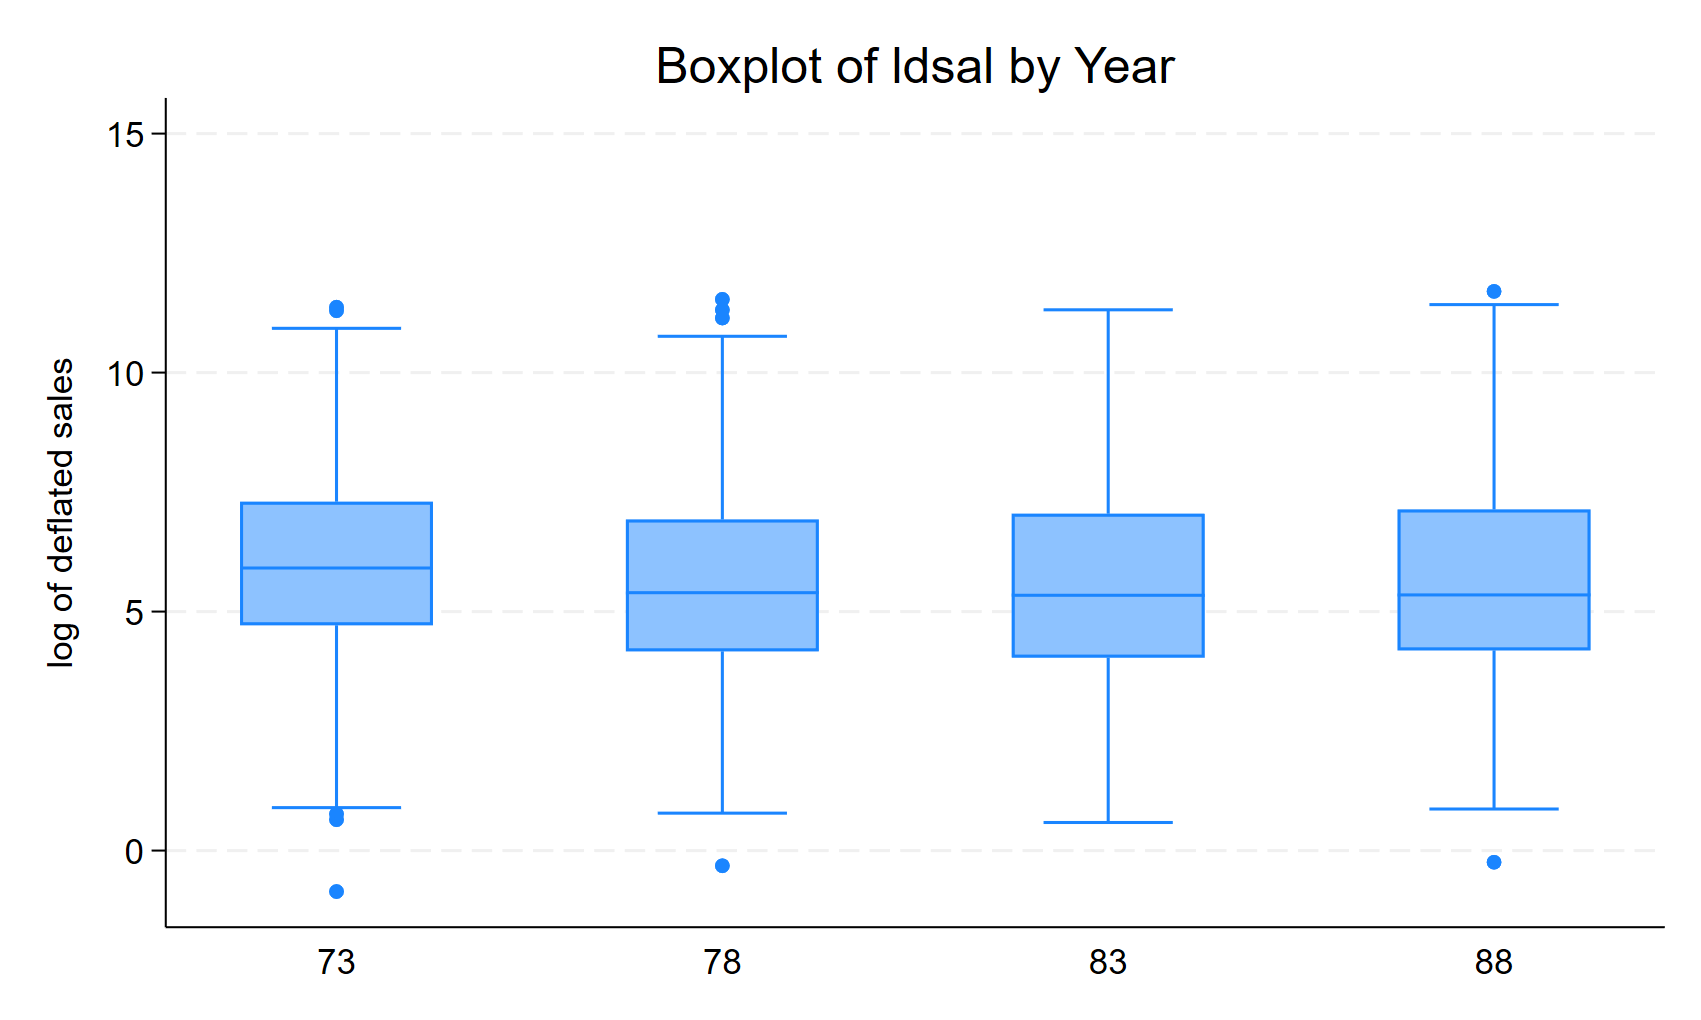
\includegraphics[width=0.8\textwidth]{boxplot_ldsal.png}
    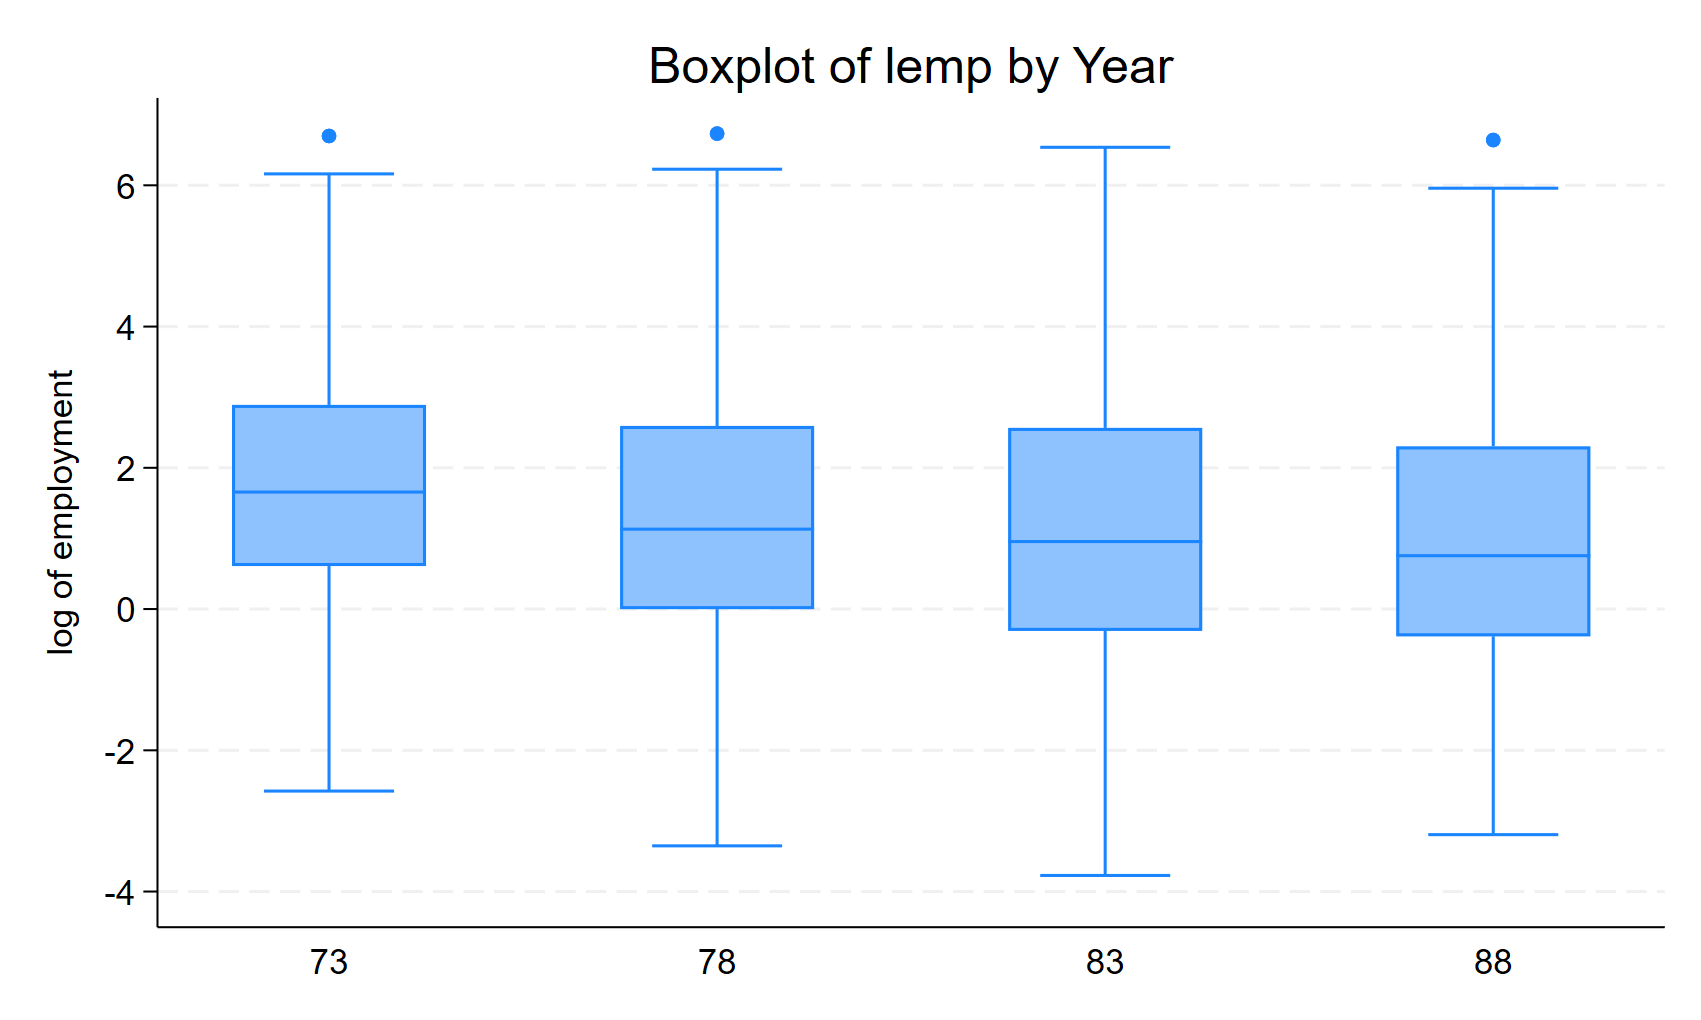
\includegraphics[width=0.8\textwidth]{boxplot_lemp.png} 
    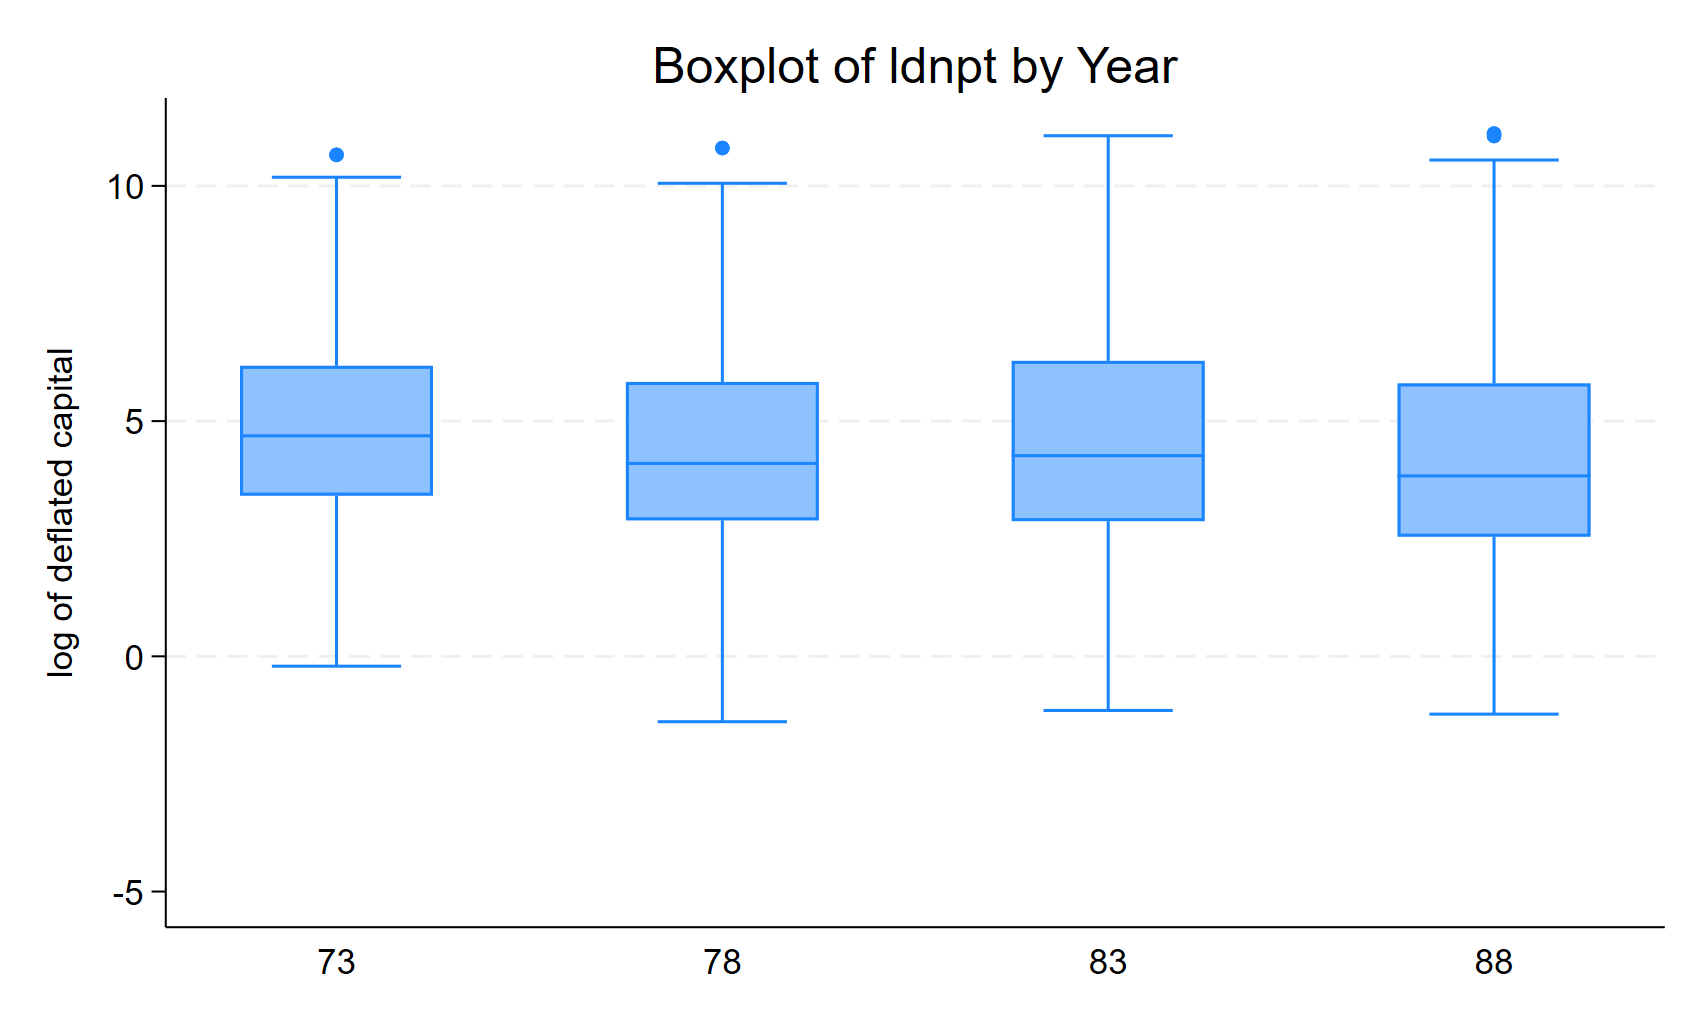
\includegraphics[width=0.8\textwidth]{boxplot_ldnpt.png} 
\end{figure}
  

\begin{lstlisting}[language=stata] 
use GMdata.dta, clear
tabstat ldsal lemp ldnpt, statistics(mean median sd min max p5 p95) by(yr)
    
graph box ldsal, over(yr) title("Boxplot of ldsal by Year")
graph export "boxplot_ldsal.png", replace
    
graph box lemp, over(yr) title("Boxplot of lemp by Year")
graph export "boxplot_lemp.png", replace
    
graph box ldnpt, over(yr) title("Boxplot of ldnpt by Year")
graph export "boxplot_ldnpt.png", replace
\end{lstlisting}

\begin{itemize}
    \item \textbf{Summary Statistics by Year:} For each year, detailed summaries (mean, median, standard deviation, minimum, maximum, 5th percentile, and 95th percentile) are computed for \texttt{ldsal}, \texttt{lemp}, and \texttt{ldnpt}.
    \item \textbf{Findings:}
    \begin{itemize}
        \item \emph{1973:} Average log-sales around 6.00, with a median of 5.91; labor and capital show relatively high values.
        \item \emph{1978:} A slight dip is observed in log-sales, and both labor and capital statistics indicate a reduction.
        \item \emph{1983:} Similar levels to 1978 with very low values at the 5th percentile for capital.
        \item \emph{1988:} A modest rebound in log-sales is observed along with a continuation of the decline in typical labor and capital values, although high outliers emerge.
    \end{itemize}
    \item \textbf{Box Plots:} Side-by-side box plots for each variable across the years reveal:
    \begin{itemize}
        \item For \texttt{ldsal}: Median sales dip in the late 1970s and early 1980s then rise by 1988, with an increasing number of high-value outliers.
        \item For \texttt{lemp}: A downward trend in median employment, indicating that the typical firm employs fewer workers in later years.
        \item For \texttt{ldnpt}: A similar downward drift in capital, with consistent high-capital outliers.
    \end{itemize}
    \item \textbf{Conclusion:} There is no clear monotonic trend in output; however, the distributions of labor and capital suggest a shift towards smaller firms in later years, while a few firms experienced very high sales by 1988.
\end{itemize}
\end{autosolution}

\begin{autosolution}
    \     

    1,186 firms are dropped when constructing a balanced panel.
\begin{lstlisting}[language=stata]
egen tag = tag(index)
count if tag == 1
local total_firms = r(N)
display "Total number of firms in the unbalanced panel: " `total_firms'
    
bysort index: egen n_obs = count(yr)
    
list index n_obs if n_obs < 4, sepby(index)
    
keep if n_obs == 4
    
egen tag_bal = tag(index)
count if tag_bal == 1
local balanced_firms = r(N)
display "Number of firms in the balanced panel: " `balanced_firms'
    
local lost_firms = `total_firms' - `balanced_firms'
display "Number of firms dropped when creating a balanced panel: " `lost_firms' 
\end{lstlisting}

\end{autosolution}

\begin{autosolution}
\

Consider the panel data model
\[
\text{ldsal}_{it} = \alpha_i + \beta_1\,\text{lemp}_{it} + \beta_2\,\text{ldnpt}_{it} + u_{it}, \quad i=1,\dots, N,\; t=1,\dots, T,
\]
where $\alpha_i$ is an unobserved firm-specific effect and $u_{it}$ is an idiosyncratic error term. In the random effects (RE) framework, $\alpha_i$ is treated as a random variable that is uncorrelated with the regressors $\text{lemp}_{it}$ and $\text{ldnpt}_{it}$.

\underline{1. Model Reformulation}

Define the composite error term as
\[
\varepsilon_{it} = \alpha_i + u_{it} - \beta_0.
\]
Thus, the model can be rewritten as
\[
\text{ldsal}_{it} = \beta_0 + \beta_1\,\text{lemp}_{it} + \beta_2\,\text{ldnpt}_{it} + \varepsilon_{it},
\]
with $\beta_0$ being an overall intercept (if included).

\underline{2. Error Structure}

Under RE, the variance of the composite error is:
\[
\operatorname{Var}(\varepsilon_{it}) = \sigma^2_\alpha + \sigma^2_u,
\]
and for two different time periods $t \neq s$ for the same firm, the covariance is:
\[
\operatorname{Cov}(\varepsilon_{it}, \varepsilon_{is}) = \sigma^2_\alpha.
\]
This intra-firm correlation suggests the use of Generalized Least Squares (GLS).

\underline{3. Quasi-Demeaning Transformation}

To account for the correlation in the error structure, a quasi-demeaning transformation is applied. For each firm $i$, define the time averages:
\[
\bar{y}_i = \frac{1}{T}\sum_{t=1}^{T} \text{ldsal}_{it}, \quad \bar{x}_i = \frac{1}{T}\sum_{t=1}^{T} x_{it},
\]
where $x_{it}$ represents each regressor (i.e., $\text{lemp}_{it}$ and $\text{ldnpt}_{it}$).

The transformed variables are:
\[
y^*_{it} = \text{ldsal}_{it} - \theta\,\bar{y}_i, \quad x^*_{it} = x_{it} - \theta\,\bar{x}_i,
\]
with the transformation parameter $\theta$ defined as:
\[
\theta = 1 - \sqrt{\frac{\sigma^2_u}{\sigma^2_u + T\sigma^2_\alpha}}.
\]
After this transformation, the model becomes:
\[
y^*_{it} = \beta_0(1-\theta) + \beta_1\,\text{lemp}^*_{it} + \beta_2\,\text{ldnpt}^*_{it} + \varepsilon^*_{it}.
\]
Applying ordinary least squares (OLS) to the transformed model yields the RE estimator:
\[
\hat{\beta}_{RE} = \left(\sum_{i=1}^{N}\sum_{t=1}^{T} x^*_{it}x^{*\prime}_{it}\right)^{-1}\left(\sum_{i=1}^{N}\sum_{t=1}^{T} x^*_{it}y^*_{it}\right).
\]

\underline{4. Assumptions for Consistency}

For the RE estimator to be consistent, the following assumptions must hold:
\begin{enumerate}
    \item \textbf{Exogeneity:} 
    \[
    E\left[u_{it} \mid \text{lemp}_{i1}, \text{ldnpt}_{i1}, \dots, \text{lemp}_{iT}, \text{ldnpt}_{iT}, \alpha_i\right] = 0.
    \]
    Equivalently, the regressors are uncorrelated with both the idiosyncratic error $u_{it}$ and the individual effect $\alpha_i$.
    
    \item \textbf{Independence of Individual Effects and Regressors:}
    \[
    E\left[\alpha_i \mid \text{lemp}_{it}, \text{ldnpt}_{it}\right] = 0 \quad \text{for all } t.
    \]
    
    \item \textbf{Homoskedasticity and No Serial Correlation:}  
    The idiosyncratic errors $u_{it}$ are assumed to be homoskedastic and serially uncorrelated (conditional on $\alpha_i$).
    
    \item \textbf{Correct Specification:}  
    The model is correctly specified with no omitted variables that are correlated with the regressors.
\end{enumerate}

\underline{5. Discussion}

In many empirical applications such as in production function estimation (e.g., Griliches and Mairesse, 1995), the assumption that $\alpha_i$ is uncorrelated with the inputs might be unrealistic. If there exists correlation between $\alpha_i$ and the regressors, the RE estimator will be inconsistent, and alternative methods like the Fixed Effects estimator should be considered.

\begin{itemize}
    \item The RE estimator is obtained by running a pooled OLS regression where the firm-specific effect $\alpha_i$ is absorbed into the error term.
    \item \textbf{Results (balanced panel):}
    \begin{table}[htbp]\centering
\def\sym#1{\ifmmode^{#1}\else\(^{#1}\)\fi}
\caption{Question (c): Random Effects Estimator}
\begin{tabular}{l*{2}{cc}}
\toprule
                    &\multicolumn{2}{c}{(1)}  &\multicolumn{2}{c}{(2)}  \\
                    &\multicolumn{2}{c}{RE}   &\multicolumn{2}{c}{RE Robust}\\
                    &           b&          se&           b&          se\\
\midrule
log of employment   &       0.509&       0.037&       0.509&       0.041\\
log of deflated capital&       0.484&       0.029&       0.484&       0.035\\
\midrule
Observations        &         856&            &         856&            \\
\bottomrule
\end{tabular}
\end{table}

    \begin{itemize}
        % \item Intercept: approximately 2.724.
        \item $\beta_1$ (Labor elasticity): about 0.509.
        \item $\beta_2$ (Capital elasticity): about 0.484.
    \end{itemize}
    \item \textbf{Interpretation:} A 1\% increase in labor is associated with a $0.5087\%$ increase in sales, and a 1\% increase in capital with a $0.4839\%$ increase in sales. The sum (approximately 0.989) is close to constant returns.
    \item \textbf{Assumptions:} Consistency requires that the unobserved firm effect $\alpha_i$ is uncorrelated with both \texttt{lemp} and \texttt{ldnpt}. This is likely violated since more productive firms may choose different input levels.
\end{itemize}

\begin{lstlisting}[language=Stata]
xtset index yr

xtreg ldsal lemp ldnpt, re
xtreg ldsal lemp ldnpt, re vce(robust)
\end{lstlisting}

\end{autosolution}

\begin{autosolution}
\    

To eliminate the unobserved firm-specific effect \(\alpha_i\), we apply the within (time-demeaning) transformation. Define the time averages for each firm \(i\) as:
\[
\bar{y}_i = \frac{1}{T}\sum_{t=1}^{T}\text{ldsal}_{it}, \quad \bar{x}_{i1} = \frac{1}{T}\sum_{t=1}^{T}\text{lemp}_{it}, \quad \bar{x}_{i2} = \frac{1}{T}\sum_{t=1}^{T}\text{ldnpt}_{it},
\]
and
\[
\bar{u}_i = \frac{1}{T}\sum_{t=1}^{T}u_{it}.
\]

Subtracting these averages from the original model gives:
\[
\text{ldsal}_{it} - \bar{y}_i = \beta_1\Bigl(\text{lemp}_{it} - \bar{x}_{i1}\Bigr) + \beta_2\Bigl(\text{ldnpt}_{it} - \bar{x}_{i2}\Bigr) + \Bigl(u_{it} - \bar{u}_i\Bigr).
\]
Let the demeaned variables be:
\[
\tilde{y}_{it} = \text{ldsal}_{it} - \bar{y}_i, \quad \tilde{\text{lemp}}_{it} = \text{lemp}_{it} - \bar{x}_{i1}, \quad \tilde{\text{ldnpt}}_{it} = \text{ldnpt}_{it} - \bar{x}_{i2},
\]
and
\[
\tilde{u}_{it} = u_{it} - \bar{u}_i.
\]

Thus, the transformed model is:
\[
\tilde{y}_{it} = \beta_1\,\tilde{\text{lemp}}_{it} + \beta_2\,\tilde{\text{ldnpt}}_{it} + \tilde{u}_{it}.
\]

The FE within estimator is obtained by applying Ordinary Least Squares (OLS) to the demeaned model:
\[
\hat{\beta}_{FE} = \left( \sum_{i=1}^{N}\sum_{t=1}^{T} \tilde{x}_{it}\tilde{x}_{it}' \right)^{-1}\left( \sum_{i=1}^{N}\sum_{t=1}^{T} \tilde{x}_{it}\tilde{y}_{it} \right),
\]
where \(\tilde{x}_{it} = \begin{pmatrix}\tilde{\text{lemp}}_{it} \\ \tilde{\text{ldnpt}}_{it}\end{pmatrix}\).

\underline{Assumptions for Consistency}

For the FE estimator to be consistent, the following assumptions must hold:
\begin{enumerate}
    \item \textbf{Strict Exogeneity:} 
    \[
    E\Bigl(u_{it}\mid \text{lemp}_{i1}, \text{ldnpt}_{i1}, \dots, \text{lemp}_{iT}, \text{ldnpt}_{iT}, \alpha_i\Bigr)=0 \quad \text{for all } t.
    \]
    \item \textbf{No Perfect Collinearity:} The demeaned regressors \(\tilde{\text{lemp}}_{it}\) and \(\tilde{\text{ldnpt}}_{it}\) are not perfectly collinear.
    \item \textbf{Large Number of Cross-Sections:} Consistency is achieved as \(N \to \infty\) while \(T\) remains fixed.
\end{enumerate}

Under these conditions, the FE estimator is consistent even if the individual effects \(\alpha_i\) are correlated with the regressors in the original model.

\begin{itemize}
    \item The FE-W estimator is computed by demeaning the data to remove the firm-specific effect $\alpha_i$.
    \item \textbf{Results (balanced panel):}
    \begin{table}[htbp]\centering
\def\sym#1{\ifmmode^{#1}\else\(^{#1}\)\fi}
\caption{Question (d): Fixed Effects (Within) Estimator}
\begin{tabular}{l*{2}{cc}}
\toprule
                    &\multicolumn{2}{c}{(1)}  &\multicolumn{2}{c}{(2)}  \\
                    &\multicolumn{2}{c}{FE}   &\multicolumn{2}{c}{FE Robust}\\
                    &           b&          se&           b&          se\\
\midrule
log of employment   &       0.765&       0.062&       0.765&       0.079\\
log of deflated capital&       0.408&       0.047&       0.408&       0.060\\
\midrule
Observations        &         856&            &         856&            \\
\bottomrule
\end{tabular}
\end{table}

    \begin{itemize}
        \item $\beta_1$: approximately 0.765.
        \item $\beta_2$: approximately 0.408.
    \end{itemize}
    \item \textbf{Interpretation:} Within a firm, a 1\% increase in labor results in about a 0.765\% increase in sales, and a 1\% increase in capital results in about a 0.408\% increase in sales. The sum (approximately 1.17) suggests increasing returns to scale in the within-firm variation.
    \item \textbf{Assumptions:} Requires strict exogeneity of the error term (i.e., no feedback from shocks to future inputs) after controlling for $\alpha_i$. Although more realistic than RE, this condition may still be violated in practice.
\end{itemize}

\begin{lstlisting}[language=Stata]
xtreg ldsal lemp ldnpt, fe
xtreg ldsal lemp ldnpt, fe vce(robust)

\end{lstlisting}

\end{autosolution}

\begin{autosolution}
\

To eliminate the unobserved firm-specific effect \(\alpha_i\), we take first differences. For \(t \geq 2\), define the first-differenced variables as:
\[
\Delta \text{ldsal}_{it} = \text{ldsal}_{it} - \text{ldsal}_{i,t-1},
\]
\[
\Delta \text{lemp}_{it} = \text{lemp}_{it} - \text{lemp}_{i,t-1}, \quad \Delta \text{ldnpt}_{it} = \text{ldnpt}_{it} - \text{ldnpt}_{i,t-1},
\]
\[
\Delta u_{it} = u_{it} - u_{i,t-1}.
\]
Then, the differenced model is given by:
\[
\Delta \text{ldsal}_{it} = \beta_1\,\Delta \text{lemp}_{it} + \beta_2\,\Delta \text{ldnpt}_{it} + \Delta u_{it}.
\]
Denote \(\Delta y_{it} = \Delta \text{ldsal}_{it}\) and
\[
\Delta x_{it} = \begin{pmatrix} \Delta \text{lemp}_{it} \\ \Delta \text{ldnpt}_{it} \end{pmatrix}.
\]
The FE First Difference estimator is then:
\[
\hat{\beta}_{FD} = \left( \sum_{i=1}^{N}\sum_{t=2}^{T} \Delta x_{it}\,\Delta x_{it}' \right)^{-1}\left( \sum_{i=1}^{N}\sum_{t=2}^{T} \Delta x_{it}\,\Delta y_{it} \right).
\]

For \(\hat{\beta}_{FD}\) to be consistent, the following assumptions are required:
\begin{enumerate}
    \item \textbf{Strict Exogeneity in Differences:}  
    \[
    E\left(\Delta u_{it} \mid \Delta x_{i1}, \Delta x_{i2}, \dots, \Delta x_{iT}\right) = 0 \quad \text{for all } t.
    \]
    \item \textbf{No Perfect Collinearity:} The differenced regressors must not be perfectly collinear.
    \item \textbf{Large Number of Cross-Sections:} The estimator is consistent as \(N \to \infty\) while \(T\) remains fixed.
\end{enumerate}


\begin{itemize}
    \item The FE-FD estimator is obtained by differencing consecutive observations, eliminating $\alpha_i$.
    \item \textbf{Results (balanced panel):}
    \begin{table}[htbp]\centering
\def\sym#1{\ifmmode^{#1}\else\(^{#1}\)\fi}
\caption{Question (e): Fixed Effects (FD) Estimator}
\begin{tabular}{l*{2}{cc}}
\toprule
                    &\multicolumn{2}{c}{(1)}  &\multicolumn{2}{c}{(2)}  \\
                    &\multicolumn{2}{c}{D\_ldsal}&\multicolumn{2}{c}{D\_ldsal}\\
                    &           b&          se&           b&          se\\
\midrule
D\_lemp              &       0.928&       0.056&       0.928&       0.066\\
D\_ldnpt             &       0.003&       0.040&       0.003&       0.046\\
\midrule
Observations        &         642&            &         642&            \\
\bottomrule
\end{tabular}
\end{table}

    \begin{itemize}
        \item $\beta_1$: approximately 0.928.
        \item $\beta_2$: approximately 0.003.
    \end{itemize}
    \item \textbf{Interpretation:} Year-to-year changes indicate that a 1\% increase in labor is associated with about a 0.928\% increase in sales, while a 1\% increase in capital is associated with only a 0.003\% increase. The large difference in capital elasticity compared to the FE-W estimator may suggest that capital adjustments have a slower or more complex dynamic in the short-run.
    \item \textbf{Assumptions:} Consistency depends on the absence of serial correlation in the errors and that changes in inputs are not influenced by past shocks.
\end{itemize}
\begin{lstlisting}[language=stata]
use "GMdata_balanced.dta", clear
sort index yr
    
by index: gen D_ldsal = ldsal - ldsal[_n-1]
by index: gen D_lemp = lemp - lemp[_n-1]
by index: gen D_ldnpt = ldnpt - ldnpt[_n-1]
    
by index: drop if _n==1

reg D_ldsal D_lemp D_ldnpt, robust
eststo fd_robust
    
reg D_ldsal D_lemp D_ldnpt, vce(cluster index)
eststo fd_robust_cluster
    
esttab fd_robust fd_robust_cluster using question_e.tex, replace label booktabs title("Question (e): Fixed Effects (FD) Estimator") ///
    cells("b(fmt(3)) se(fmt(3))") keep(D_lemp D_ldnpt)    
\end{lstlisting}
\end{autosolution}


\begin{autosolution}   
\

Define the time-demeaned variables as:
\[
\tilde{y}_{it} = y_{it} - \bar{y}_i,\quad \tilde{x}_{it} = x_{it} - \bar{x}_i,
\]
with
\[
\bar{y}_i = \frac{1}{T}\sum_{t=1}^{T} y_{it},\quad \bar{x}_i = \frac{1}{T}\sum_{t=1}^{T} x_{it}.
\]
Then the transformed model becomes:
\[
\tilde{y}_{it} = \tilde{x}_{it}'\beta + \tilde{u}_{it}, \quad \text{where}\quad \tilde{u}_{it} = u_{it} - \bar{u}_i.
\]

The Fixed Effects (FE) estimator is given by:
\[
\hat{\beta}_{FE} = \left(\sum_{i=1}^{N}\sum_{t=1}^{T}\tilde{x}_{it}\tilde{x}_{it}'\right)^{-1}\left(\sum_{i=1}^{N}\sum_{t=1}^{T}\tilde{x}_{it}\tilde{y}_{it}\right).
\]
Since \(\tilde{y}_{it} = \tilde{x}_{it}'\beta + \tilde{u}_{it}\), we have:
\[
\hat{\beta}_{FE} - \beta = \left(\sum_{i=1}^{N}\sum_{t=1}^{T}\tilde{x}_{it}\tilde{x}_{it}'\right)^{-1}\left(\sum_{i=1}^{N}\sum_{t=1}^{T}\tilde{x}_{it}\tilde{u}_{it}\right).
\]

Under standard regularity conditions, and with \(T\) fixed and \(N \to \infty\), it holds that:
\[
\frac{1}{NT}\sum_{i=1}^{N}\sum_{t=1}^{T}\tilde{x}_{it}\tilde{x}_{it}' \stackrel{p}{\to} Q,
\]
and
\[
\frac{1}{\sqrt{N}} \sum_{i=1}^{N}\sum_{t=1}^{T}\tilde{x}_{it}\tilde{u}_{it} \stackrel{d}{\to} N(0, \Sigma),
\]
where
\[
Q = E\left[\frac{1}{T}\sum_{t=1}^{T}\tilde{x}_{it}\tilde{x}_{it}'\right],
\]
and
\[
\Sigma = \operatorname{Var}\left(\frac{1}{\sqrt{T}}\sum_{t=1}^{T}\tilde{x}_{it}\tilde{u}_{it}\right).
\]

Hence, by Slutsky's theorem,
\[
\sqrt{N}(\hat{\beta}_{FE} - \beta) = \left(\frac{1}{NT}\sum_{i=1}^{N}\sum_{t=1}^{T}\tilde{x}_{it}\tilde{x}_{it}'\right)^{-1} \left(\frac{1}{\sqrt{N}} \sum_{i=1}^{N}\sum_{t=1}^{T}\tilde{x}_{it}\tilde{u}_{it}\right)
\]
converges in distribution to:
\[
\sqrt{N}(\hat{\beta}_{FE} - \beta) \stackrel{d}{\to} N\Bigl(0,\, Q^{-1}\Sigma Q^{-1}\Bigr).
\]
\end{autosolution}

\begin{autosolution}   
\

Recall from the asymptotic distribution of the FE estimator that
\[
\sqrt{N}(\hat{\beta}_{FE} - \beta) \xrightarrow{d} N\Bigl(0,\, Q^{-1}\Sigma Q^{-1}\Bigr),
\]
where
\[
Q = \lim_{N\to\infty}\frac{1}{NT}\sum_{i=1}^{N}\sum_{t=1}^{T}\tilde{x}_{it}\tilde{x}_{it}', \quad
\Sigma = \lim_{N\to\infty}\operatorname{Var}\left(\frac{1}{\sqrt{N}}\sum_{i=1}^{N}\sum_{t=1}^{T}\tilde{x}_{it}\tilde{u}_{it}\right).
\]
An estimator for the asymptotic variance of \(\hat{\beta}_{FE}\) is given by:
\[
\widehat{\operatorname{Var}}(\hat{\beta}_{FE}) = \left(\sum_{i=1}^{N}\sum_{t=1}^{T}\tilde{x}_{it}\tilde{x}_{it}'\right)^{-1}\left(\sum_{i=1}^{N}\sum_{t=1}^{T}\tilde{x}_{it}\tilde{x}_{it}'\hat{u}_{it}^2\right)
\left(\sum_{i=1}^{N}\sum_{t=1}^{T}\tilde{x}_{it}\tilde{x}_{it}'\right)^{-1},
\]
where \(\hat{u}_{it}\) are the residuals from the FE regression. Consequently, the standard error for the \(j\)th coefficient is given by:
\[
\text{se}(\hat{\beta}_{j}) = \sqrt{\left[\widehat{\operatorname{Var}}(\hat{\beta}_{FE})\right]_{jj}}.
\]
This robust variance estimator is used in empirical software to report standard errors that are consistent even under heteroscedasticity and autocorrelation of the error term.

\begin{itemize}
    \item The robust (clustered) standard errors are computed using the formula
    \[
    \hat{V} = \widehat{Q}^{-1} \widehat{\Sigma}\, \widehat{Q}^{-1},
    \]
    where \(\widehat{\Sigma} = \frac{1}{N}\sum_{i=1}^{N} X_i^{*\prime}\hat{u}_i \hat{u}_i' X_i^*\).
    \item With the balanced panel, the estimated standard errors are approximately:
    \begin{itemize}
        \item SE\((\hat{\beta}_1) \approx 0.079\),
        \item SE\((\hat{\beta}_2) \approx 0.060\).
    \end{itemize}
    \begin{table}[htbp]\centering
\def\sym#1{\ifmmode^{#1}\else\(^{#1}\)\fi}
\caption{Question (g): FE Regression with Robust SE}
\begin{tabular}{l*{1}{cc}}
\toprule
                    &\multicolumn{2}{c}{(1)}  \\
                    &\multicolumn{2}{c}{log of deflated sales}\\
                    &           b&          se\\
\midrule
log of employment   &       0.765&       0.079\\
log of deflated capital&       0.408&       0.060\\
\midrule
Observations        &         856&            \\
\bottomrule
\end{tabular}
\end{table}

    \item These values indicate high statistical significance of the estimated coefficients.
\end{itemize}

\begin{lstlisting}[language=stata]
xtreg ldsal lemp ldnpt, fe robust
\end{lstlisting}

\end{autosolution}

\begin{autosolution}
\

Consider a balanced panel with \(N\) firms and \(T\) time periods per firm. The Fixed Effects (FE) estimator is obtained by first demeaning the data:
\[
\tilde{y}_{it} = y_{it} - \bar{y}_i,\quad \tilde{x}_{it} = x_{it} - \bar{x}_i,
\]
where
\[
\bar{y}_i = \frac{1}{T}\sum_{t=1}^{T}y_{it}, \quad \bar{x}_i = \frac{1}{T}\sum_{t=1}^{T}x_{it}.
\]
The FE estimator is then given by
\[
\hat{\beta} = \left(\sum_{i=1}^{N}\sum_{t=1}^{T}\tilde{x}_{it}\tilde{x}_{it}'\right)^{-1}\left(\sum_{i=1}^{N}\sum_{t=1}^{T}\tilde{x}_{it}\tilde{y}_{it}\right).
\]

To account for within-firm correlation and obtain robust standard error estimates, we employ a clustered bootstrap procedure as follows:

\begin{enumerate}
    \item \textbf{Resampling:} For \(b=1,\dots,B\) (with \(B=1000\)), draw a bootstrap sample by resampling \(N\) firms with replacement from the original sample. For each selected firm, include all \(T\) observations.
    
    \item \textbf{Estimation:} Compute the FE estimator on the bootstrap sample to obtain \(\hat{\beta}^{*(b)}\).
    
    \item \textbf{Variance Estimation:} The bootstrap estimator for the variance of \(\hat{\beta}\) is
    \[
    \widehat{\operatorname{Var}}_{\text{boot}}(\hat{\beta}) = \frac{1}{B-1}\sum_{b=1}^{B}\left(\hat{\beta}^{*(b)} - \bar{\hat{\beta}}^{*}\right)\left(\hat{\beta}^{*(b)} - \bar{\hat{\beta}}^{*}\right)',
    \]
    where
    \[
    \bar{\hat{\beta}}^{*} = \frac{1}{B}\sum_{b=1}^{B}\hat{\beta}^{*(b)}.
    \]
    
    \item \textbf{Standard Errors:} The standard error for the \(j\)th coefficient is
    \[
    \text{se}(\hat{\beta}_{j}) = \sqrt{\left[\widehat{\operatorname{Var}}_{\text{boot}}(\hat{\beta})\right]_{jj}}.
    \]
\end{enumerate}

This clustered bootstrap procedure yields standard error estimates that are robust to within-cluster (firm) correlation.

\begin{itemize}
    \begin{table}[htbp]\centering
\def\sym#1{\ifmmode^{#1}\else\(^{#1}\)\fi}
\caption{Question (h): FE Bootstrap Estimates (Manual)}
\begin{tabular}{l*{1}{cc}}
\toprule
                    &\multicolumn{2}{c}{(1)}  \\
                    &\multicolumn{2}{c}{}     \\
                    &           b&          se\\
\midrule
\_bs\_1               &       0.765&       0.080\\
\_bs\_2               &       0.408&       0.060\\
\midrule
Observations        &         856&            \\
\bottomrule
\end{tabular}
\end{table}

    \item The clustered bootstrap resamples firms (clusters) with replacement, preserving the panel structure.
    \item With \(B = 1000\) bootstrap replications, the bootstrap standard errors are found to be:
    \begin{itemize}
        \item SE\((\hat{\beta}_1) \approx 0.080\),
        \item SE\((\hat{\beta}_2) \approx 0.060\).
    \end{itemize}
    \item The bootstrap results confirm the accuracy of the analytical cluster-robust standard errors.
\end{itemize}

\begin{lstlisting}[language=stata]
use "GMdata_balanced.dta", clear

program define fe_est, rclass
    preserve
    bysort index: egen ymean = mean(ldsal)
    bysort index: egen x1mean = mean(lemp)
    bysort index: egen x2mean = mean(ldnpt)

    gen yd = ldsal - ymean
    gen x1d = lemp - x1mean
    gen x2d = ldnpt - x2mean

    quietly regress yd x1d x2d, noconstant
    return scalar b1 = _b[x1d]
    return scalar b2 = _b[x2d]
    restore
end

bootstrap r(b1) r(b2), reps(1000) cluster(index) nodots: fe_est
    
\end{lstlisting}

\end{autosolution}

\begin{autosolution}
\

Consider the panel data model:
\[
y_{it} = \alpha_i + x_{it}'\beta + u_{it}, \quad i=1,\dots,N,\; t\in \mathcal{T}_i,
\]
where \( \mathcal{T}_i \) denotes the set of time periods for which firm \( i \) is observed and \( T_i = |\mathcal{T}_i| \).

For each firm \( i \), define the time averages based on the available observations:
\[
\bar{y}_i = \frac{1}{T_i}\sum_{t\in \mathcal{T}_i} y_{it}, \quad \bar{x}_i = \frac{1}{T_i}\sum_{t\in \mathcal{T}_i} x_{it}.
\]
The within (demeaning) transformation yields:
\[
\tilde{y}_{it} = y_{it} - \bar{y}_i, \quad \tilde{x}_{it} = x_{it} - \bar{x}_i, \quad t\in \mathcal{T}_i.
\]

The transformed model is:
\[
\tilde{y}_{it} = \tilde{x}_{it}'\beta + \tilde{u}_{it}, \quad \text{with} \quad \tilde{u}_{it} = u_{it} - \bar{u}_i,
\]
and
\[
\bar{u}_i = \frac{1}{T_i}\sum_{t\in \mathcal{T}_i} u_{it}.
\]

The Fixed Effects (FE) estimator is then given by:
\[
\hat{\beta}_{FE} = \left( \sum_{i=1}^{N}\sum_{t\in \mathcal{T}_i} \tilde{x}_{it}\tilde{x}_{it}' \right)^{-1} \left( \sum_{i=1}^{N}\sum_{t\in \mathcal{T}_i} \tilde{x}_{it}\tilde{y}_{it} \right).
\]
Under standard assumptions (strict exogeneity, no perfect collinearity, etc.), \(\hat{\beta}_{FE}\) is consistent for \(\beta\) even when the panel is unbalanced.

\begin{itemize}
    \item The full dataset (unbalanced panel) is used to re-estimate the FE model.
    \item \textbf{Results (unbalanced panel):}
    \begin{table}[htbp]\centering
\def\sym#1{\ifmmode^{#1}\else\(^{#1}\)\fi}
\caption{Question (i): FE Estimator on Unbalanced Panel}
\begin{tabular}{l*{2}{cc}}
\toprule
                    &\multicolumn{2}{c}{(1)}  &\multicolumn{2}{c}{(2)}  \\
                    &\multicolumn{2}{c}{FE}   &\multicolumn{2}{c}{FE Robust}\\
                    &           b&          se&           b&          se\\
\midrule
log of employment   &       0.753&       0.035&       0.753&       0.061\\
log of deflated capital&       0.311&       0.026&       0.311&       0.037\\
\midrule
Observations        &        2971&            &        2971&            \\
\bottomrule
\end{tabular}
\end{table}

    \begin{itemize}
        \item \(\beta_1 \approx 0.753\) with a clustered standard error of about 0.061.
        \item \(\beta_2 \approx 0.311\) with a clustered standard error of about 0.037.
    \end{itemize}
    \item \textbf{Interpretation:} Compared to the balanced panel, the labor coefficient is similar, but the capital coefficient is lower. This may reflect sample selection effects; firms with incomplete data (often newer or smaller firms) exhibit lower capital productivity.
\end{itemize}

\begin{lstlisting}[language=stata]
use "GMdata.dta", clear
xtset index yr
    
xtreg ldsal lemp ldnpt, fe
    
xtreg ldsal lemp ldnpt, fe vce(robust)
    
\end{lstlisting}
\end{autosolution}

\begin{autosolution}
\    

Let \(\hat{\beta}_{FE}\) be the Fixed Effects (FE) estimator obtained from the original panel data model:
\[
y_{it} = \alpha_i + x_{it}'\beta + u_{it}, \quad i=1,\dots,N,\; t\in \mathcal{T}_i.
\]
For each firm \(i\), define the time-demeaned variables as:
\[
\tilde{y}_{it} = y_{it} - \bar{y}_i,\quad \tilde{x}_{it} = x_{it} - \bar{x}_i,
\]
with
\[
\bar{y}_i = \frac{1}{T_i}\sum_{t\in \mathcal{T}_i} y_{it}, \quad \bar{x}_i = \frac{1}{T_i}\sum_{t\in \mathcal{T}_i} x_{it}.
\]
The FE estimator is then given by:
\[
\hat{\beta}_{FE} = \left(\sum_{i=1}^{N}\sum_{t\in \mathcal{T}_i}\tilde{x}_{it}\tilde{x}_{it}'\right)^{-1}\left(\sum_{i=1}^{N}\sum_{t\in \mathcal{T}_i}\tilde{x}_{it}\tilde{y}_{it}\right).
\]

To account for within-firm correlation, we use a clustered bootstrap procedure:
\begin{enumerate}
    \item \textbf{Resampling:} For \(b = 1, \dots, B\) (with \(B = 1000\)), draw a bootstrap sample by sampling \(N\) firms with replacement from the original data. For each selected firm, include all \(T_i\) observations.
    
    \item \textbf{Estimation:} Compute the FE estimator on the \(b\)th bootstrap sample to obtain \(\hat{\beta}_{FE}^{*(b)}\).
    
    \item \textbf{Bootstrap Variance:} The variance of \(\hat{\beta}_{FE}\) is estimated by
    \[
    \widehat{\operatorname{Var}}_{\text{boot}}(\hat{\beta}_{FE}) = \frac{1}{B-1}\sum_{b=1}^{B}\left(\hat{\beta}_{FE}^{*(b)} - \bar{\hat{\beta}}^{*}\right)\left(\hat{\beta}_{FE}^{*(b)} - \bar{\hat{\beta}}^{*}\right)',
    \]
    where
    \[
    \bar{\hat{\beta}}^{*} = \frac{1}{B}\sum_{b=1}^{B} \hat{\beta}_{FE}^{*(b)}.
    \]
    
    \item \textbf{Standard Errors:} The standard error for the \(j\)th coefficient is given by
    \[
    \text{se}(\hat{\beta}_{j}) = \sqrt{\left[\widehat{\operatorname{Var}}_{\text{boot}}(\hat{\beta}_{FE})\right]_{jj}}.
    \]
\end{enumerate}

This clustered bootstrap method provides standard error estimates that are robust to intra-cluster (firm-level) correlation.

\begin{itemize}
    \begin{table}[htbp]\centering
\def\sym#1{\ifmmode^{#1}\else\(^{#1}\)\fi}
\caption{Question (j): FE Bootstrap on Unbalanced Panel (Manual)}
\begin{tabular}{l*{1}{cc}}
\toprule
                    &\multicolumn{2}{c}{(1)}  \\
                    &\multicolumn{2}{c}{}     \\
                    &           b&          se\\
\midrule
\_bs\_1               &       0.753&       0.058\\
\_bs\_2               &       0.311&       0.037\\
\midrule
Observations        &        2971&            \\
\bottomrule
\end{tabular}
\end{table}

    \item The clustered bootstrap is also applied to the unbalanced panel.
    \item With \(B=1000\) replications, the bootstrapped standard errors are approximately:
    \begin{itemize}
        \item SE\((\hat{\beta}_1) \approx 0.058\),
        \item SE\((\hat{\beta}_2) \approx 0.037\).
    \end{itemize}
    \item These values closely match the analytical robust standard errors, reinforcing the robustness of our estimates.
\end{itemize}
\end{autosolution}

\begin{lstlisting}[language=stata]
use "GMdata.dta", clear
xtset index yr
    
program define fe_est2, rclass
    preserve
    bysort index: egen ymean2 = mean(ldsal)
    bysort index: egen x1mean2 = mean(lemp)
    bysort index: egen x2mean2 = mean(ldnpt)

    gen yd2 = ldsal - ymean2
    gen x1d2 = lemp - x1mean2
    gen x2d2 = ldnpt - x2mean2

    quietly regress yd2 x1d2 x2d2, noconstant
    return scalar b1 = _b[x1d2]
    return scalar b2 = _b[x2d2]
    restore
end
    
bootstrap r(b1) r(b2), reps(1000) cluster(index) nodots: fe_est2
\end{lstlisting}

\end{document}

